\exercise{Timer}
Si realizzi la classe \cod{Timer} che svolga le funzioni di cronometro. Tale oggetto deve poter gestire i messaggi START, STOP, RESET e GETTIME comportandosi come specificato dall'interfaccia seguente.

\begin{methodslist}

\method{start}{\emptyset}{\emptyset}{
Avvia il conteggio del tempo.
}

\method{stop}{\emptyset}{\emptyset}{
Arresta il conteggio del tempo.
}

\method{reset}{\emptyset}{\emptyset}{
Arresta ed azzera il timer.
}

\method{getTime}{\emptyset}{int}{
Restituisce il conteggio corrente del tempo in secondi.
}

\end{methodslist}

Nella figura � riportato un esempio grafico del funzionamento dell'oggetto.

\begin{figure}
  \center
	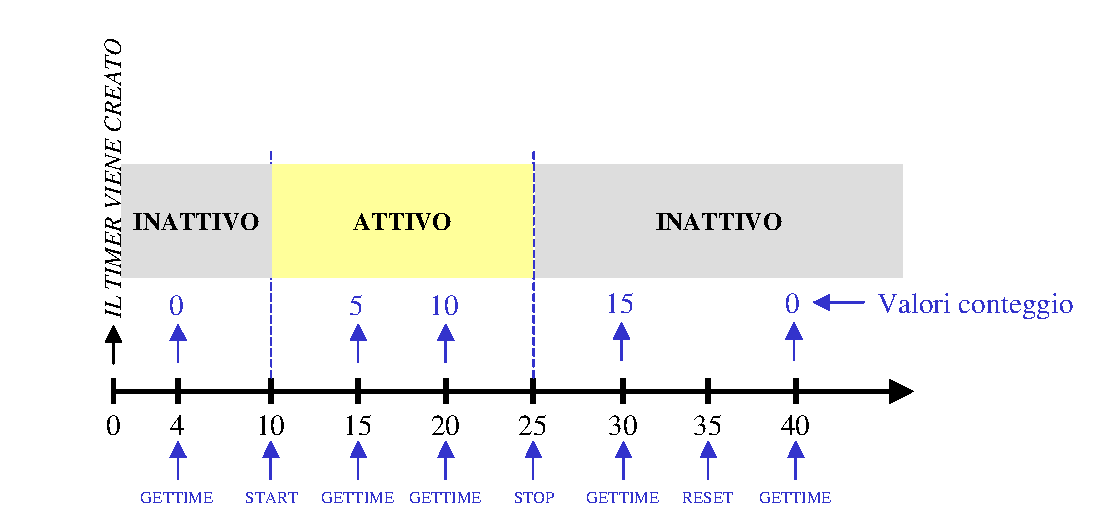
\includegraphics[width=.9\textwidth]{Esercizi/Timer/Timer.eps}
	\caption{Un esempio d'uso del timer nel tempo}
	\label{fig:Timer}	
\end{figure}

Si realizzi una classe \cod{Main} dotata di un metodo \cod{main()} che permetta di effettuare il collaudo della struttura dati realizzata.

Nessuno dei metodi della classe pu� operare con i canali di input/output (per es. \cod{System.out}). L'interfacciamento con l'utente per la lettura e la visualizzazione dei dati sono concessi esclusivamente all'interno della classe \cod{Main}.

\subsubsection*{Suggerimenti}
\begin{itemize}
\item
Le classi standard \cod{java.\-time.\-Local\-Date\-Time} e \cod{java.\-time.\-Duration} implementano il trattamento delle date e delle durate temporali. Consultando la documentazione di queste classi � possibile conoscere i servizi messi da queste a disposizione. Per esempio, la chiamata al metodo \cod{LocalDateTime.now()} restituisce un'istanza della classe \cod{java.\-time.\-Local\-Date\-Time} contenente l'ora corrente del sistema.
\item
Il funzionamento del timer nei casi non espressamente previsti dalle specifiche sia arbitrario.
\end{itemize}